\documentclass[aspectratio=169]{beamer}
\usetheme{singapore}
\usecolortheme{default}

\usepackage{hyperref}
\usepackage{setspace}
\usepackage{graphicx}
\usepackage{lscape}
\usepackage{tikz}
\usepackage{pgfplots}
\usepackage{amsmath}
\usepackage{esdiff}
\usepackage{float}
\usepackage{tabularx}
\usepackage{caption}
\usepackage{subcaption}

\usepackage{environ}

\newlength{\myl}
\expandafter\let\expandafter\origequation\csname equation*\endcsname
\expandafter\let\expandafter\endorigequation\csname endequation*\endcsname
\long\def\[#1\]{\begin{equation*}#1\end{equation*}}
\RenewEnviron{equation*}{
	\settowidth{\myl}{$\displaystyle\BODY$} % calculate width and save as \myl
	\origequation
	\ifdim\myl>\linewidth
	\resizebox{\linewidth}{!}{$\displaystyle\BODY$}% \myl > \linewidth
	\else
	\BODY % \myl <= \linewidth
	\fi
	\endorigequation
}

\title[Bias in VE Estimation]{How Important Are Study Designs?}
\subtitle{A Simulation Approach in Assessing Bias in VE Estimation with Time-Varying Vaccine Coverage, and Heterogeneous Testing and Baseline Attack Rates}
\author{Jing Lian Suah${}^a$ \qquad Naor Bar-Zeev${}^b$ \qquad Masliyana Husin${}^a$ \\ Boon Hwa Tng${}^a$ \qquad Maria Deloria Knoll${}^b\dagger$ \qquad Sheamini Sivasampu${}^a\dagger$}
\institute[ICR \& JHU]{${}^a$Institute for Clinical Research, National Institutes of Health, Malaysia \\ ${}^b$Bloomberg School of Public Health, John Hopkins University \\ $\dagger$ Co-Senior Authors}
\date{\today}

\begin{document}
	
\begin{frame}
	\titlepage
	\begin{center}
		\tiny
		Any views expressed are that of the researchers, and should not be taken to represent those of the Government of Malaysia
	\end{center}
\end{frame}	

\section{Highlights}
\begin{frame}{Highlights}
	\small
	\begin{itemize}
		\item This paper simulated a \textbf{theoretical model with frictions in vaccination, testing, baseline disease risks, and heterogeneous vaccine effectiveness} to evaluate estimation bias across \textbf{four cohort and two test-negative designs}.
		\item In theory, \textbf{bias depends on behavioural asymmetries} (in testing, and baseline risk) between the vax-willing and vax-unwilling, and the \textbf{speed of vaccination rollout}.
		\item Even under `ideal' conditions (no frictions), there is \textbf{intrinsic estimation bias} across all study designs of different magnitudes.
		\item In scenarios that may be reflective of past SARS-CoV-2 waves, the \textbf{degree of bias can be substantial}, attributable to variation in assumed testing and baseline risk frictions. 
		\item A formal regression-based decomposition indicates that study designs have visibly \textbf{different primary sources of estimation bias, and degree of robustness} in general.
		\item This study warrants a \textbf{re-benchmarking of methodology and reporting checklists} for VE research, and informs the design of cost-effective surveillance by \textbf{quantifying part of the bias-implementation cost trade-off}.
	\end{itemize}
\end{frame}

\section{Research Question}
\begin{frame}{Research Question and Approach}
	\begin{block}{Research Question}
		How do commonly used VE study designs (variations of cohorts, and TNDs) perform in the presence of (i) time-varying vaccine coverage, (ii) latent selection of testing and risk behaviours on willingness to vaccinate, and (iii) `leaky' vaccines?
	\end{block}
	\begin{block}{Analytical Steps}
		\begin{enumerate}
			\item Deriving an expression for the theoretical bias in a conceptual model of the epidemiological environment
			\item Simulate data using the conceptual model, and compute the VE estimation bias under various configurations of cohorts and TNDs
			\item Analyse the relative importance of the various drivers of bias
		\end{enumerate}
	\end{block}
\end{frame}

\begin{frame}{Logic of the entire study}
	\centering 
	\footnotesize
	
	$k$ parameter sets $\Xi = (\Xi_1 \ \Xi_2 \ \Xi_3 \ ... \ \Xi_k)$, as \textbf{input}, which contains the mean of the VE distribution, $\mu_{VE}$, which is used to calculate estimation bias ($\widehat{VE} - \mu_{VE}$) \\
	
	$\Downarrow$ \\
	
	Set up a \textbf{theoretical model} detailing the `epidemiological environment' as a function $f(\centerdot)$, which describes how people get vaccinated, get tested, develop outcomes (generalisable), and how vaccines confer protection at the individual- \& population-levels, etc \\
	
	$\Downarrow$ \\ 
	
	Use the theoretical model $f$ to \textbf{simulate data} from every parameter set in $\Xi$, producing $k$ sets of simulated data ($y_k)$; use \textbf{parallel processing} to speed up computation \\ 
	
	$\Downarrow$ \\ 
	
	For every set of simulated data $y_k$, \textbf{estimate VE} using $M$ study designs (variations of cohorts and TNDs), and \textbf{calculate the respective estimation bias} \\
	
	$\Downarrow$ \\ 
	
	Concatenate all of the estimation biases by study designs, and parameter sets for \textbf{specific analysis} \\
	
	\begin{minipage}{0.32\linewidth}
		\centering 
		$\Downarrow$ \\ 
		\textbf{Scenario analysis: }Zoom into special parameter sets e.g., similar to SARS-CoV-2 waves
	\end{minipage}
	\begin{minipage}{0.32\linewidth}
		\centering 
		$\Downarrow$ \\ 
		\textbf{Drivers decomposition: }Linear regression to analyse relative importance of sources of bias
	\end{minipage}
	\begin{minipage}{0.32\linewidth}
		\centering 
		$\Downarrow$ \\ 
		\textbf{Relative ranks (Additional): }Compute stability of relative bias between study designs
	\end{minipage}
\end{frame}

\begin{frame}{Computational logistics of the study}
	\begin{itemize}
		\item The simulation was run on a AWS EC2 c6i.32xLarge Amazon Linux instance (128 vCPUs), which took \textbf{415516 seconds (115.42 hours)}. 
		\begin{itemize}
			\item Running on a Windows 10, 4-core (8 logical processors) 11th gen i5 local machine would have taken\textbf{ at least 1154 hours (48 days)}, subject to sufficient memory.
			\item Virtual machines can be expensive! This means that stress tests, fail-safes, and minimum working examples need to be implemented thoroughly beforehand. 
		\end{itemize}
		\item Post-simulation analyses were run on Windows 10, 4-core (8 logical processors) 10th gen i7 local machine, as no parallel processing is required.
	\end{itemize}
\end{frame}

\section{Conceptual Model \& Simulation}
\begin{frame}{Key assumptions of the theoretical model}
	\footnotesize
	\begin{enumerate}
		\item Vaccination coverage at least increases over time (vaccination rollout is either pre-completed, or ongoing throughout the study)
		\item A share of the population is vaccination-willing (\textit{vax-willing}; conversely vaccination-unwilling or \textit{vax-unwilling}) but may not necessarily receive the vaccine
		\item A share of the population is test-willing (conversely, test-unwilling) but may not necessarily test for the disease
		\item The vax-unwilling's probability of testing, suppose test-willing, may differ from that of the vax-willing
		\item Vaccine effectiveness differs between individuals, but is distributed along a particular mean/mode
		\item Suppose not yet infected, then the risk of infection follows a memoryless process
		\item All individuals can be infected at most once, hence no re-infections
		\item The baseline infection risk of the vax-unwilling may differ from that of the vax-willing
	\end{enumerate}
\textbf{Hence, there are four groups --- } (1) Vax-willing and test-willing, (2) Vax-willing but test-unwilling, (3) Vax-unwilling but test-willing, (4) Vax-unwilling and test-unwilling
\end{frame}

\begin{frame}{There are 10 parameters in the model ($888125$ valid combinations)}
\begin{table}[H]
	\begin{center}
		\resizebox*{!}{0.8\textheight}{
		\begin{tabular}{||p{0.15\linewidth}| p{\linewidth}|p{0.28\linewidth}||}
			\hline \hline
			\textbf{Parameter} & \textbf{Meaning} & \textbf{Values for Simulation} \\
			\hline \hline 
			$N$ & Simulated population size & 1000 \\
			\hline 
			$T$ & Number of time periods used in the simulation; this is equivalent to the follow-up duration & 20, 30, 40, 50, 60 \\
			\hline 
			$\Theta_{v}$ & Fraction of population that is willing to be vaccinated (vax-willing); fraction $\Theta_{v}$ takes values $\theta_{v} = 1$ and fraction $1 - \Theta_{v}$ takes values $\theta_{v} = 0$ & 0.3, 0.4, 0.5, 0.6, 0.7 \\
			\hline 
			$p_v$ & Probability of being vaccinated if not already vaccinated but vax-willing in period $t$; $p_v=1$ implies static coverage, such that all vax-willing start off vaccinated, and $p_v \rightarrow 0$ the opposite &  0.15, 0.3, 0.4, 0.5, 0.6, 0.85, 1 \\
			\hline 
			$\Theta_{\tau}$ & Fraction of population that is willing to be tested (test-willing); fraction $\Theta_{\tau}$ takes values $\theta_{\tau} = 1$ and fraction $1 - \Theta_{\tau}$ takes values $\theta_{\tau} = 0$ & 0.5, 0.65, 0.75, 0.85, 1 \\
			\hline 
			$p_\tau$ & Probability of being tested if test-willing in period $t$ & 0.5, 0.65, 0.75, 0.85, 1 \\
			\hline 
			$k_\tau$ & Ratio of probability of being tested of the vax-unwilling to the vax-willing ($\frac{p_\tau^{\theta_{v}=0}}{p_\tau^{\theta_{v}=1}}$); $k_\tau < 1$ indicates that the vax-unwilling are less likely to be tested than the vax-willing & 0.5, 0.75, 0.9, 1, 1.1, 1.25, 1.5 \\
			\hline 
			$\alpha_{b}$ & Baseline attack rate for the vax-willing, which is the daily probability of contracting the disease if vax-willing but unvaccinated & 0.025 \\
			\hline 
			$k_\alpha$ & Ratio of the baseline infection rate of the vax-unwilling relative to that of the vax-willing ($\frac{\alpha_{b}^{\theta_{v}=0}}{\alpha_{b}}$); $k_\alpha < 1$ indicates that the baseline infection rate of the vax-unwilling is lower than that of the vax-willing & 0.5, 0.75, 0.9, 1, 1.1, 1.25, 1.5 \\
			\hline 
			$\mu_{VE}$ & Mean of the VE distribution, ${VE}_{i} \sim Beta(\alpha=9,\beta=\frac{\alpha}{\mu_{VE}} - \alpha), \ 0 < \mu_{VE} < 1$ for individual $i$ & 0.5, 0.6, 0.7, 0.8, 0.9 \\
			\hline \hline
		\end{tabular}
	}
	\end{center}
\end{table}
\end{frame}

\begin{frame}{Bias is decreasing in $p_v$, and increases as $k_{\tau}$ and $k_{\alpha}$ diverge from $1$}
	\tiny
	\begin{eqnarray}
		{Bias}\{\widehat{VE}\} = \widehat{VE} - VE = \sum_{t=0}^{T} w_{t} \bigg( \frac{\Theta_{v} ( 1 - \Theta_{v} ) \phi_v \phi_{uv}' ( \Omega' - \Omega ) }{\big( \Theta_{v} \phi_{uv} + (1 - \Theta_{v}) \phi_{uv}'  \big) \big( \Theta_{v} \phi_{uv} \Omega + ( 1 - \Theta_{v}) \phi_{uv}' \Omega' \big)} \bigg) \\ 
		\textbf{where} \ VE = \sum_{t=0}^{T} w_{t} VE_{t} = \sum_{t=0}^{T} w_{t} \Big( 1 - \frac{\Theta_{v}\phi_v}{\Theta_{v} \phi_{uv} + (1 - \Theta_{v}) \phi_{uv}' } \Big) \\
		\textbf{and} \ \widehat{VE} = \sum_{t=0}^{T} w_{t} \widehat{VE}_{t} = \sum_{t=0}^{T} w_{t} \Big( 1 - \frac{\Theta_{v}\phi_v\Theta_{\tau}\Omega }{\Theta_{v} \phi_{uv}\Theta_{\tau}\Omega + (1 - \Theta_{v}) \phi_{uv}'\Theta_{\tau}\Omega' } \Big) \\ 
		\textbf{and} \ \phi_v = \sum_{m}^{t-1} (1-p_v)^{t-1-m} p_v \sum_{n}^{t-1}(1-\alpha_{uv})^{n}(1-\alpha_{v})^{t-1-n}\alpha_{v} \\
		\textbf{and} \ \phi_{uv} = \sum_{m}^{t} (1-p_v)^{m} \sum_{n}^{t-1} (1-\alpha_{uv})^{n}\alpha_{uv} \\
		\textbf{and} \ \phi_{uv}' = \sum_{m}^{t-1} (1- k_\alpha \alpha_{uv})^{m} k_\alpha \alpha_{uv} \\
		\textbf{and} \ \Omega = j(p_\tau) = \sum_{m}^{t} p_{\tau} \sum_{n}^{t-1} (1-p_{\tau})^{n}p_{\tau} \sum_{q}^{t-1} (1-p_{\tau})p_{\tau}^{q} \sum_{r}^{t-1} (1-p_{\tau})^{t-1-r} p_{\tau}^{r} \\ 
		\textbf{and} \ \Omega' = j(k_\tau p_\tau) = \sum_{m}^{t} k_{\tau} p_{\tau} \sum_{n}^{t-1} (1- k_{\tau} p_{\tau})^{n} k_{\tau} p_{\tau} \sum_{q}^{t-1} (1- k_{\tau} p_{\tau}) k_{\tau} p_{\tau}^{q} \sum_{r}^{t-1} (1- k_{\tau} p_{\tau})^{t-1-r} (k_{\tau} p_{\tau})^{r}
	\end{eqnarray}
\end{frame}

\begin{frame}{Interpreting the theoretical bias equation}
	\begin{itemize}
		\item Bias is a function of the behavioural asymmetries between the vax-willing and vax-unwilling ($\Theta_{\tau}$, $p_\tau$, and $k_\tau$), and the speed of vaccination rollout ($p_v$)
		\item Unambiguously, if the testing behaviour of the vax-willing and vax-unwilling are identical ($k_\tau = 1$, hence $\Omega = \Omega'$), then theoretical bias is nil
		\item The prevalence of test-willing individuals ($\Theta_{\tau}$) does not matter, but the prevalence of vax-willing ($\Theta_{v}$) matters
	\end{itemize}
\end{frame}

\begin{frame}{Simulation focuses on commonly used cohorts and test-negative designs}
	\begin{table}[H]
		\begin{center}
			\resizebox*{!}{0.8\textheight}{
				\begin{tabular}{||p{0.4\linewidth}|p{0.3\linewidth}| p{0.7\linewidth}||}
					\hline \hline
					\textbf{Study Design} & \textbf{Estimation Approach} & \textbf{Notes} \\
					\hline \hline
					Cohort using aggregated data, with person-days as offset & Negative binomial regression (count analysis) & Commonly used where aggregate data is preferred or accessible in lieu of granular data, albeit often with a Poisson regression \\ 
					\hline
					Cohort using aggregated data, with daily population as offset & Negative binomial regression (count analysis) & Same as above but uses directly population, which may be time-varying, instead of person-days \\ 
					\hline
					Cohort using individual-level data, adjusting for immortal time bias & Cox Regression (survival analysis) & Often used in prospective cohorts where time-to-event is of interest, and where the quality of exposure-censoring time variables are robustly collected \\ 
					\hline
					Cohort using individual-level data & Logistic regression (binary outcomes) & Often used where time measures are unreliable, when time-to-event not of interest, as opposed to occurrence of outcomes, or when assumptions necessary for survival models, e.g., proportional hazards, fail \\ 
					\hline
					TND using individual-level data, keeping only the first positive, and, if never positive, the first negative test & Logistic regression (binary outcomes) & Often used when testing data from ambulatory care settings, healthcare facility screening, administrative registers, and ILI/SARI surveillance are deployed \\ 
					\hline 
					TND using individual-level data, keeping only the first positive, but allowing for multiple negative tests & Logistic regression (binary outcomes) & Used when multiple follow-up points per unique individuals are available, such as through community infection surveys \\ 
					\hline
					\hline
			\end{tabular}}
		\end{center}
	\end{table}
\end{frame}

\section{Scenario Analysis}
\begin{frame}{Scenarios to illustrate bias of existing VE estimates in practice}
	\begin{table}[H]
		\begin{center}
			\resizebox*{!}{0.8\textheight}{
			\begin{tabular}{||p{0.6\linewidth}||p{0.2\linewidth}||p{0.04\linewidth}|p{0.04\linewidth}|p{0.04\linewidth}|p{0.04\linewidth}|p{0.04\linewidth}|p{0.04\linewidth}||}
				\hline \hline
				\textbf{Scenario} & \textbf{Approximant} & $p_v$ & $\Theta_{\tau}$ & $p_\tau$ & $k_\tau$ & $k_\alpha$ & $\mu_{VE}$ \\
				\hline \hline
				\textbf{Scenario A} (Slow rollout, comprehensive testing and tracing, vax-unwilling-biased baseline risks) & Wild Type & 0.15 & 1 & 1 & 1 & 1.25 & 0.9 \\
				\hline
				\textbf{Scenario B} (Slow rollout, partly comprehensive testing and tracing, vax-unwilling-biased baseline risks) & Alpha/ Beta/ Gamma & 0.15 & 0.75 & 1 & 1 & 1.25 & 0.9 \\
				\hline
				\textbf{Scenario C} (Gradual rollout, selective testing and tracing, symmetric baseline risks) & Delta & 0.3 & 0.75 & 0.75 & 1 & 1 & 0.7 \\
				\hline
				\textbf{Scenario D} (Fast rollout, highly selective testing and tracing, vax-willing-biased baseline risks) & Omicron BA1-2 & 0.5 & 0.75 & 0.5 & 0.75 & 0.75 & 0.5\\
				\hline
				\textbf{Scenario E} (Rapid rollout, minimal testing and tracing, vax-willing-biased baseline risks) & Omicron BA3-5 & 0.85 & 0.5 & 0.5 & 0.75 & 0.75 & 0.5 \\
				\hline
				\textbf{Scenario A \& B (Severe Outcomes)} & Wild Type/ Alpha/ Beta/ Gamma & 0.15 & 1 & 1 & 1 & 1 & 0.9 \\
				\hline
				\textbf{Scenario C (Severe Outcomes)} & Delta & 0.3 & 1 & 1 & 1 & 1 & 0.9 \\
				\hline
				\textbf{Scenario D (Severe Outcomes)} & Omicron BA1-2 & 0.5 & 1 & 1 & 1 & 1 & 0.9 \\
				\hline
				\textbf{Scenario E (Severe Outcomes)} & Omicron BA3-5 & 0.85 & 1 & 1 & 1 & 1 & 0.9 \\
				\hline \hline
		\end{tabular}}
		\end{center}
	\end{table}
\end{frame}

\section{Drivers of Bias}
\begin{frame}{Estimate bias-parameter sensitivities using OLS linear regressions --- \\ (1) design-stratified, and (2) dummy fixed effects}
	\centering
	\textbf{Parameters are redefined to help interpret relative importance}
	\small
	\begin{itemize}
		\item $k_\tau$ $\rightarrow$ $|k_\tau - 1|$; absolute deviation from 1 (deviation from \textbf{independent testing rates})
		\item $p_v$ $\rightarrow$ $|p_v - 1|$; absolute shortfall from 1 (deviation from \textbf{static vaccine coverage})
		\item $p_\tau$ $\rightarrow$ $|p_\tau - 1|$; absolute shortfall from 1 (deviation from \textbf{perfect testing if test-willing})
		\item $\Theta_\tau$ $\rightarrow$ $|\Theta_\tau - 1|$; absolute shortfall from 1 (deviation from \textbf{full test-willing population})
		\item $\Theta_{v}$ $\rightarrow$ $|\Theta_{v} - 1|$; absolute shortfall from 1 (deviation from \textbf{full vax-willing population})
		\item $\mu_{VE}$ $\rightarrow$ $|\mu_{VE} - 1|$; absolute shortfall from 1 (deviation from \textbf{`perfect' vaccine})
	\end{itemize}
	\centering
	\textit{*Invariable parameters ($N$, and $\alpha_{b}$) are omitted}
	\textbf{`Ideal' conditions refers to when $p_v=1$, $\Theta_{\tau}=1$, $p_{\tau}=1$, $k_{\tau}=1$, and $k_{\alpha}=1$}
\end{frame}

\section{Findings}
\subsection{Simulation}
\begin{frame}{Under `ideal' assumptions, survival analysis and count analysis cohorts, and TNDs with multiple negative tests perform best}
	\begin{figure}[H]
		\begin{subfigure}[c]{0.31\linewidth}
			\centering
			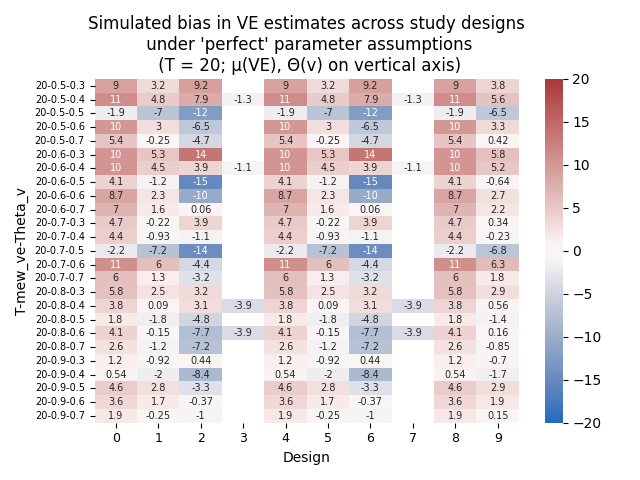
\includegraphics[scale=0.28]{VEMethod_Sim1b_PureDesignBias_Heatmap20.png}
		\end{subfigure}
		\begin{subfigure}[c]{0.31\linewidth}
			\centering
			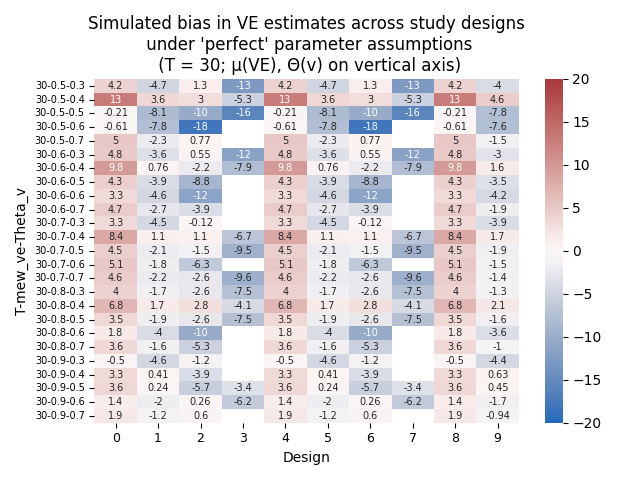
\includegraphics[scale=0.28]{VEMethod_Sim1b_PureDesignBias_Heatmap30.png}
		\end{subfigure}
		\begin{subfigure}[c]{0.31\linewidth}
			\centering
			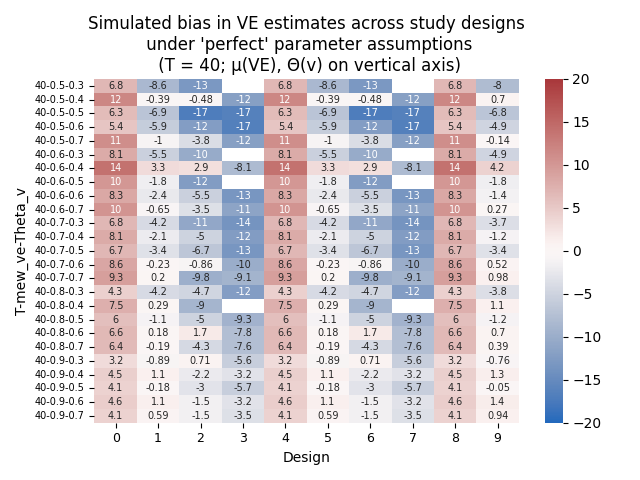
\includegraphics[scale=0.28]{VEMethod_Sim1b_PureDesignBias_Heatmap40.png}
		\end{subfigure}
	
		\begin{subfigure}[c]{0.31\linewidth}
			\centering
			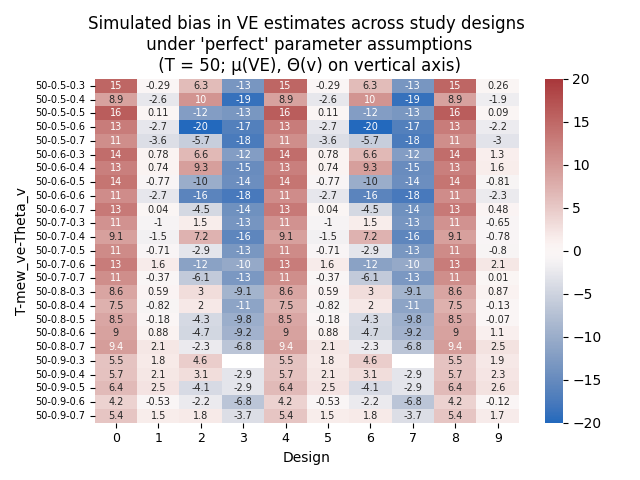
\includegraphics[scale=0.28]{VEMethod_Sim1b_PureDesignBias_Heatmap50.png}
		\end{subfigure}
		\begin{subfigure}[c]{0.31\linewidth}
			\centering
			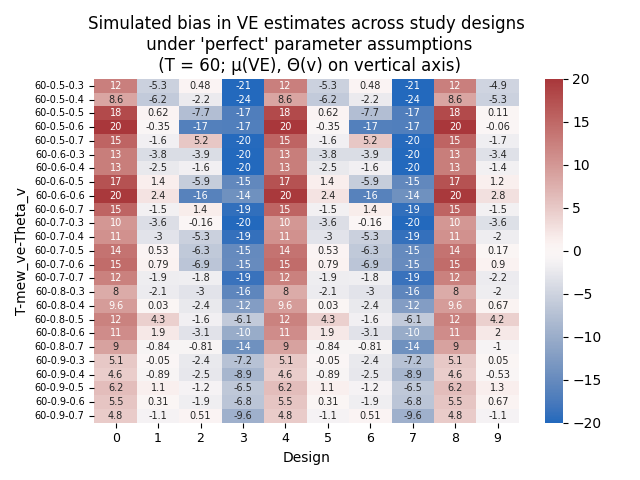
\includegraphics[scale=0.28]{VEMethod_Sim1b_PureDesignBias_Heatmap60.png}
		\end{subfigure}
		\begin{subfigure}[c]{0.31\linewidth}
			\centering
			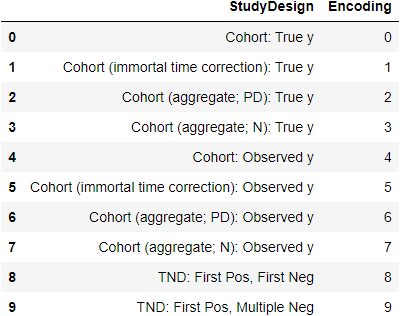
\includegraphics[scale=0.28]{VEmethod_RelDirection1b_DictDesign.png}
		\end{subfigure}
	\end{figure}
\end{frame}

\begin{frame}{Downward bias is sizeable in scenarios D and E, where deviations from `ideal' are largest, and most representative of the recent Omicron waves}
	\begin{figure}[H]
		\centering
		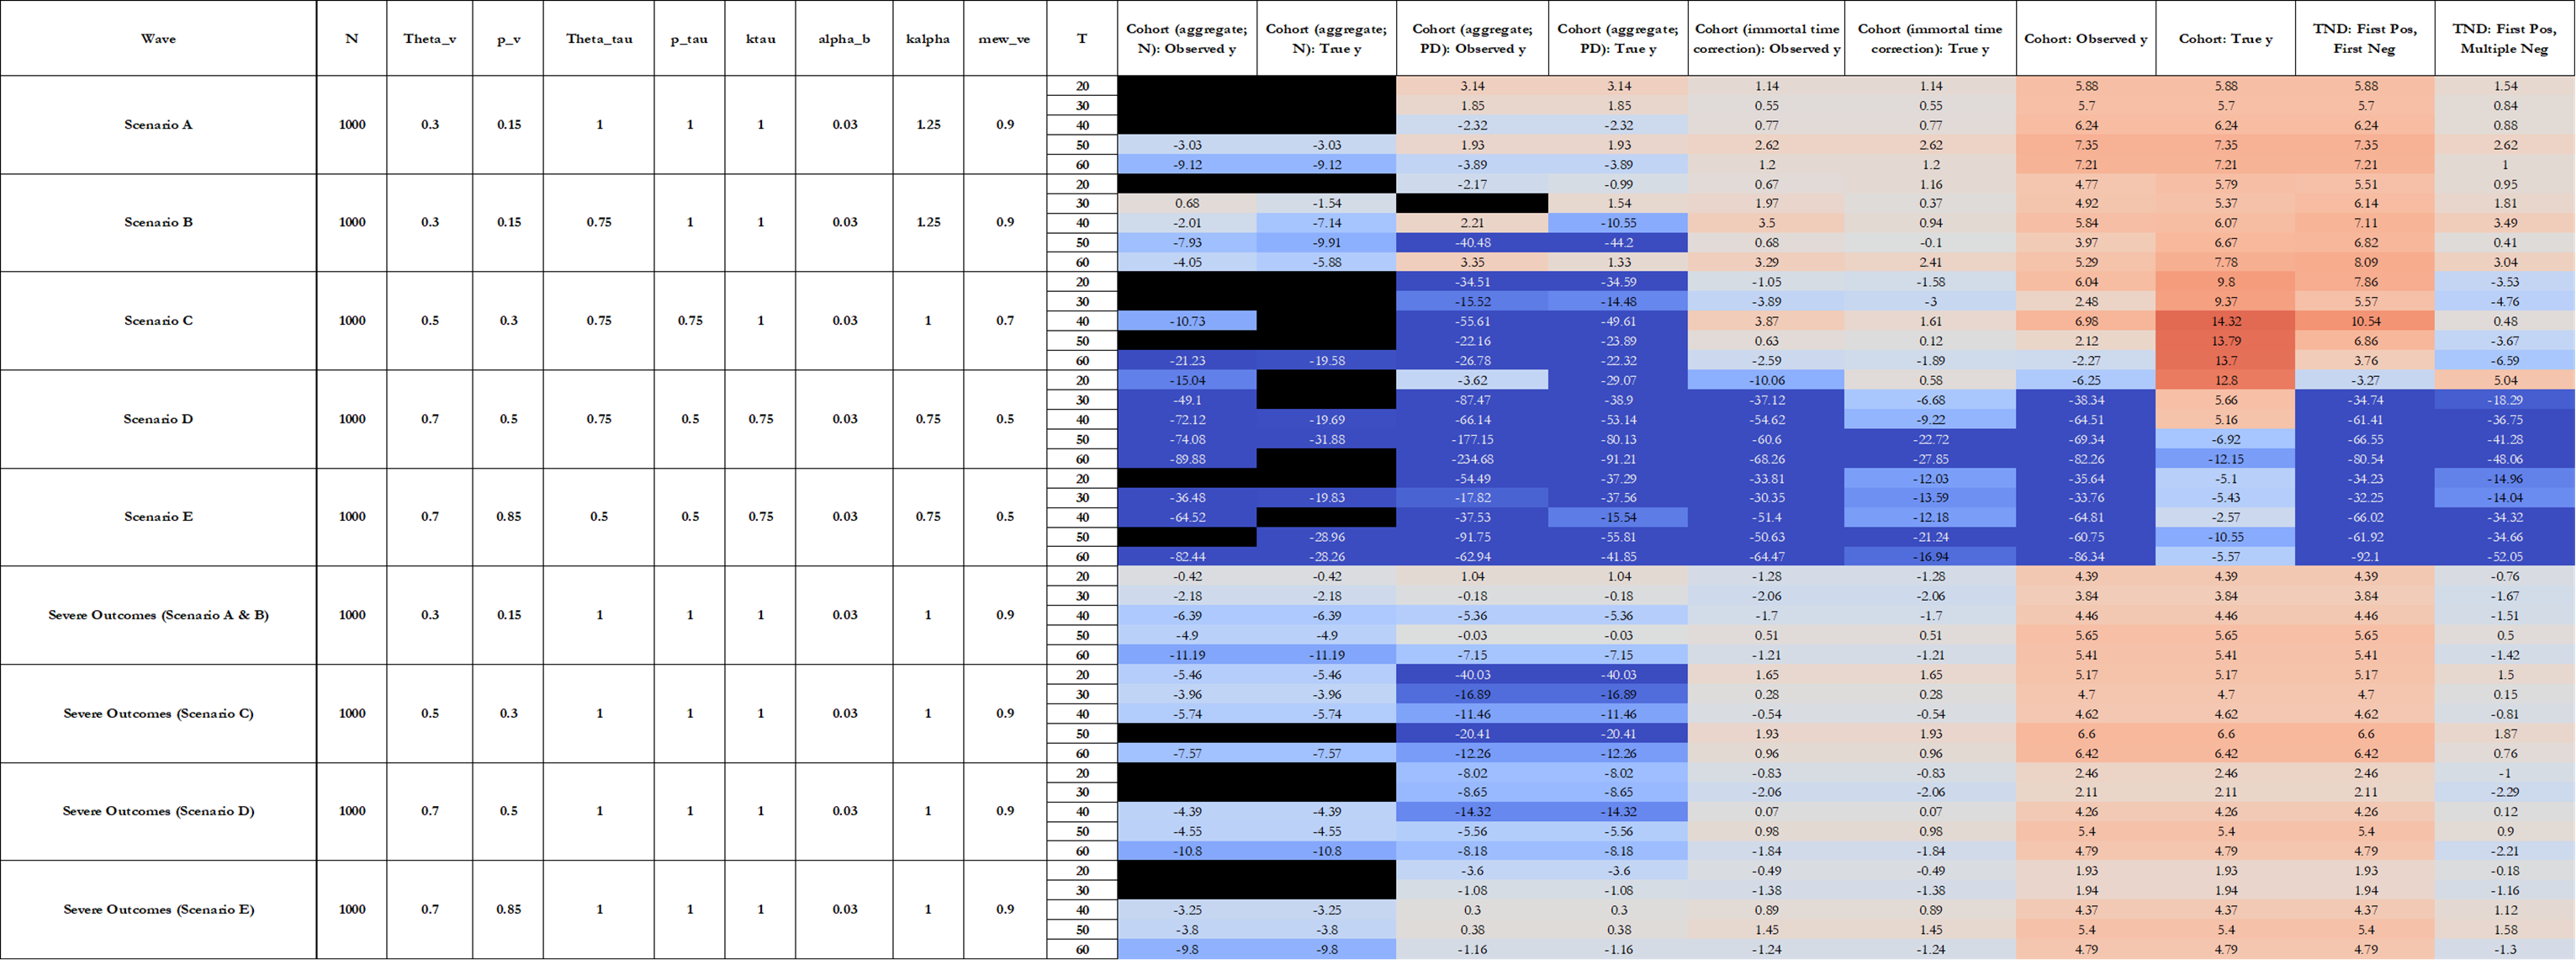
\includegraphics[scale=0.22]{VEMethod_Sim1b_WaveSpecific_Heatmap.png}
	\end{figure}
\end{frame}

\subsection{Drivers of Bias}
\begin{frame}{Summary of findings on \textbf{drivers of bias}}
	\footnotesize
	\begin{itemize}
		\item Across all study designs, the deviation in the mean of the VE distribution ($\mu_{VE}$) from `perfect' protection (100\%) exerts a downward bias; this reflects the asymmetry in the beta distribution
		\item In binary outcomes and survival analysis cohorts, $k_\tau$, and $p_\tau$ are most important. Of secondary importance are $k_\alpha$, $p_v$, $\Theta_v$, and $\Theta_{\tau}$
		\item In count analysis cohorts, $k_\tau$, $p_v$, $p_\tau$, and $\Theta_{v}$ are most important
		\item In TNDs with only one test per individual, only $k_\tau$ stood out, followed secondarily by $p_\tau$, and $k_\alpha$
		\begin{itemize}
			\scriptsize
			\item As this configuration aims to remove the influence of timing of vaccination on the risk of disease exposure, $p_v$ has a smaller association with bias; same goes for$\Theta_{\tau}$
		\end{itemize}
		\item In the TND with multiple negative tests per individual, $k_\alpha$ is important, followed secondarily by $k_\tau$, $\Theta_{v}$, and $p_v$.
		\item \textbf{Both specifications of TNDs are more robust to `less-than-ideal' conditions than cohorts, making TNDs attractive} when vaccine rollout is dynamic, and when testing is imperfect, such as during resource-constrained periods.
		\item \textit{Immense gains if steps are taken to mitigate selective testing in respective infectious disease surveillance systems, such as through randomness in community sampling.}
	\end{itemize}
\end{frame}

\begin{frame}{Decomposition of simulated bias using dummy FE and stratified OLS regression shows vast heterogeneity in the parameter-bias nexus}
	\begin{figure}[H]
		\centering
		\begin{subfigure}[t]{0.23\linewidth}
			\centering
			\includegraphics[scale=0.25]{VEMethod_Drivers1b_FEest_Li_MSpec_Heatmap5.png}
		\end{subfigure}
		\begin{subfigure}[t]{0.23\linewidth}
			\centering
			\includegraphics[scale=0.25]{VEMethod_Drivers1b_FEest_Li_MSpec_Heatmap6.png}
		\end{subfigure}
		\begin{subfigure}[t]{0.23\linewidth}
			\centering
			\includegraphics[scale=0.25]{VEMethod_Drivers1b_FEest_Li_MSpec_Heatmap7.png}
		\end{subfigure}
		\begin{subfigure}[t]{0.23\linewidth}
			\centering
			\includegraphics[scale=0.25]{VEMethod_Drivers1b_FEest_Li_MSpec_Heatmap8.png}
		\end{subfigure}
		
		\begin{subfigure}[t]{0.23\linewidth}
			\centering
			\includegraphics[scale=0.25]{VEMethod_Drivers1b_FEest_Li_MSpec_Heatmap9.png}
		\end{subfigure}
		\begin{subfigure}[t]{0.23\linewidth}
			\centering
			\includegraphics[scale=0.25]{VEMethod_Drivers1b_FEest_Li_MSpec_Heatmap10.png}
		\end{subfigure}
	\end{figure}
\end{frame}

\begin{frame}{Average and Largest Sensitivity Between Parameters $\Xi$ and Absolute Bias (Parameter With Largest Sensitivity on Vertical Axis)}
	\begin{figure}[H]
		\centering
		\includegraphics[scale=0.5]{VEMethod_Drivers1b_FEest_Li_MSpec_Robustness_Heatmap.png}
	\end{figure}
\end{frame}

\section{Discussion and Limitations}
\begin{frame}{Discussion}
	\small
	\begin{enumerate}
		\item Study design choices have \textbf{non-trivial effects on VE estimation bias}
		\item Findings warrant a \textbf{re-benchmarking of methodology}
		\begin{itemize}
			\scriptsize
			\item Recommendations for VE research need to reflect COVID-19-specific nuances
			\item Use heat maps of bias-parameter sensitivities to `adjust' VE estimates
			\item Future research ought to layout the sources of bias discussed to help form judgment on the extent of estimation bias $\rightarrow$ \textbf{additional reporting checklist}
		\end{itemize}
		\item Helps design cost-effective surveillance systems by quantifying part of the \textbf{estimation bias vs. implementation cost trade-off}
		\begin{itemize}
			\scriptsize
			\item Conceptually, the policymaker `chooses' a system that (1) mitigates sources of bias, and (2) geared towards the least biased VE study design, given resource constraint
			\item Resource-constrained countries may opt to concentrate their surveillance systems on major outbreak zones to use TNDs, rather than more resource-intensive cohorts
		\end{itemize}
		\item \textbf{Disease progression, or severity of symptoms, that is correlated with testing propensity} can be discussed within the model
		\begin{itemize}
			\scriptsize
			\item Low testing rate amongst the test-willing ($p_\tau \ll 1$) + lower testing rate amongst the vax-willing ($k_\tau \gg 1$) $\rightarrow$ symptoms tend to be milder amongst the vaccinated, hence less likely to test
		\end{itemize}
	\end{enumerate}
\end{frame}

\begin{frame}{We recommend future VE research to report the following, in addition to the STROBE checklist}
	\begin{table}[H]
		\begin{center}
			\resizebox*{!}{0.75\textheight}{
				\begin{tabular}{||p{0.04\linewidth}|p{\linewidth}|p{0.45\linewidth}||}
					\hline \hline
					\textbf{No.} & \textbf{Item} & \textbf{Purpose} \\
					\hline \hline 
					\textbf{1} & Pace of vaccination (daily time series or average) \textbf{during} the study period, including trend breaks, e.g., surge in doses given & To gauge $p_v$ \\
					\hline
					\textbf{2} & Vaccine coverage \textbf{by the end of} the study period & To gauge $\Theta_{v}$ (and potentially $k_v$) \\
					\hline
					\textbf{3} & The pace of vaccination rollout \textbf{after} the study period & To gauge $\Theta_{v}$ (and potentially $k_v$) \\
					\hline
					\textbf{4} & Testing rate in the study population, and the overall population & To gauge $\Theta_{\tau}$ and $p_\tau$ \\
					\hline
					\textbf{5} & Testing rate by vaccination status or relevant comparator groups & To gauge $k_\tau$ \\
					\hline
					\textbf{6} & Contact tracing regime (if relevant for disease studied) in place during the study period, e.g., comprehensive forward and backward, symptomatic forward only, no contact tracing & To gauge $\Theta_{\tau}$, and $p_\tau$ \\
					\hline
					\textbf{7} & Testing regime in place during the study period, including scope, eligibility, barriers of accessibility (direct and indirect), and selection criteria related to vaccination, e.g., universal (including asymptomatic) testing with private cost, symptomatic testing with private cost, symptomatic testing with price or queue discrimination on vaccination status & To gauge $\Theta_{\tau}$, $p_\tau$, and $k_\tau$ \\
					\hline
					\textbf{8} & Presence of NPIs to influence vaccine take-up via restrictions on disease transmission-relevant activities & To gauge $k_\alpha$ \\
					\hline
					\textbf{9} & \textbf{[For TNDs]} Baseline characteristics of study participants stratified by vaccination status (usually reported by test-positive, and test-negative) & To gauge $k_\alpha$, and $k_\tau$ \\
					\hline
					\textbf{10} & \textbf{[Where available]} VE estimates from meta-analyses, and systematic reviews specific to the disease, pathogenic variant, and clinical outcome of interest & To form priors on $\mu_{VE}$ beyond the study \\
					\hline \hline
				\end{tabular}
			}
		\end{center}
	\end{table}
\end{frame}

\begin{frame}{Limitations}
	\begin{enumerate}
		\item Tests with sub-100\% sensitivity and specificity is not explicitly modelled
		\begin{itemize}
			\item Reasonable sensitivities and specificities (in the region of 80\% to 90\%) $\rightarrow$ minimal bias for both cohorts and TNDs (\textit{Jackson and Rothman (2015)})
		\end{itemize}
		\item Re-infections are not explicitly modelled
		\begin{itemize}
			\item Past infections compound with vaccines $\rightarrow$ undetected infections amongst vaccinated $>$ unvaccinated $\rightarrow$ overestimate VE
		\end{itemize}
		\item Observed confounding is not explicitly modelled 
		\begin{itemize}
			\item Requires strong and non-generalisable assumptions on the structure between potential confounders, vaccination choice, and disease
		\end{itemize}
	\end{enumerate}
\end{frame}

\section{Additional Findings}
\begin{frame}{}
	\begin{block}{Additional Findings}
	\end{block}
\end{frame}

\begin{frame}{(Part 1/2) Unless indicated otherwise, range of colours $ = [-20, 20]$}
	\begin{itemize}
		\item A hypothetical 20 ppt over-estimation represents a substantial gap in estimated, and `true' protection offered.
		\item A 20 ppt over-estimation puts this the estimated COVID-19 vaccine effectiveness against death from a meta-analysis of 8 vaccine platforms spanning 5 VOCs (Higdon et al, 2022) from the neighbourhood of 60\% - 99\% to 40\% - 79\%.
		\item The equivalent for severe disease goes from 55\% - 99\% to 35\% - 79\%, and that of SARS-CoV-2 infection to well below 50\%.
	\end{itemize}
\end{frame}
\begin{frame}{(Part 2/2) Unless indicated otherwise, range of colours $ = [-20, 20]$}
	\footnotesize
	\begin{itemize}
		\item For sufficiently low baseline attack rates ($<1\%$), as is for severe COVID-19, 20 ppt can represent sizeable changes in NNV even when the estimated VE is high
	\end{itemize}
	\begin{minipage}{0.48\linewidth}
		\begin{figure}[H]
			\caption{Contour Map of NNV against VE, Conditional on $\alpha_{b}$}
			\centering
			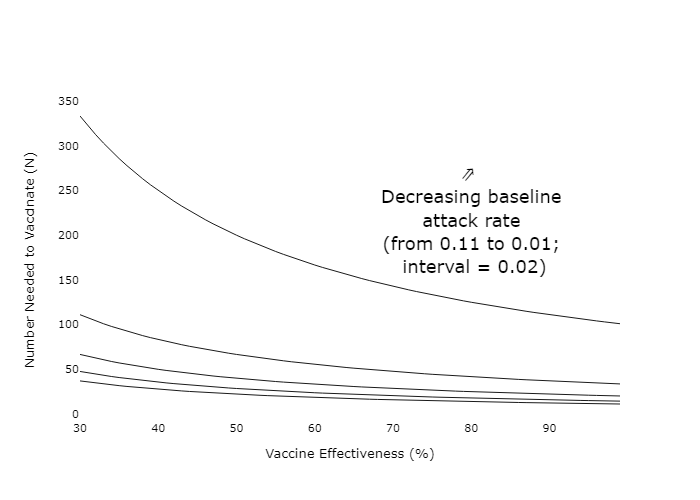
\includegraphics[scale=0.26]{VEMethod_NNVmap_NNV.png}
		\end{figure}
	\end{minipage}
	\begin{minipage}{0.48\linewidth}
		\begin{figure}[H]
			\centering
			\caption{Contour Map of first derivative of NNV against VE, Conditional on $\alpha_{b}$}
			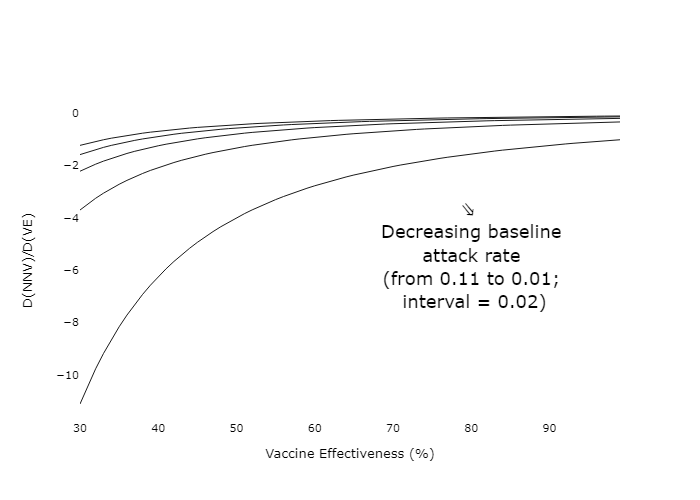
\includegraphics[scale=0.26]{VEMethod_NNVmap_Dnnv.png}
		\end{figure}
	\end{minipage}
\end{frame}

\begin{frame}{Rank reversals are common; these rankings need to consider real-world frequency of the corresponding parameter settings}
	\begin{figure}[H]
		\centering
		\begin{subfigure}[c]{0.48\linewidth}
			\centering
			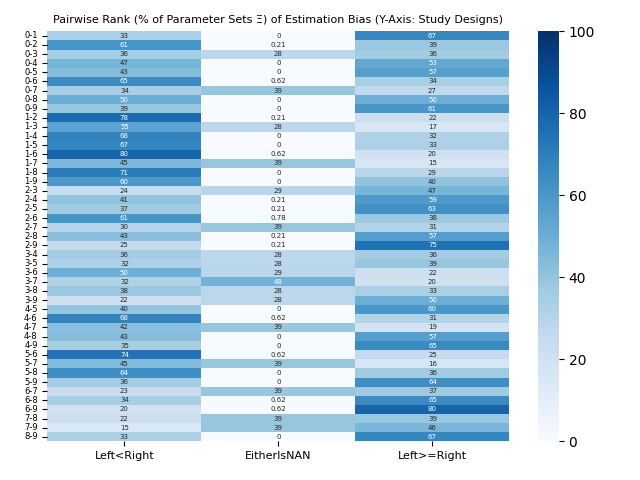
\includegraphics[scale=0.45]{VEmethod_RelDirection1b_Pairwise}
		\end{subfigure}
		\begin{subfigure}[c]{0.48\linewidth}
			\centering
			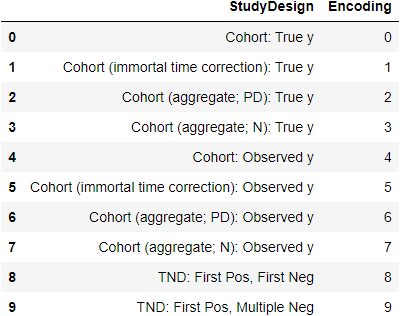
\includegraphics[scale=0.45]{VEmethod_RelDirection1b_DictDesign}
		\end{subfigure}
	\end{figure}
\end{frame}

\begin{frame}{\textbf{Rescaled (1)} Association Between Parameters $\Xi$ and Absolute Bias}
	\begin{center}
		(\textbf{Scenario D}: $p_v=0.5$; $\Theta_{\tau}=0.75$; $p_\tau=0.5$; $k_\tau=0.75$; $k_\alpha=0.75$)
	\end{center}
	\begin{figure}[H]
		\centering		
		\begin{subfigure}[t]{0.23\linewidth}
			\centering
			\includegraphics[scale=0.25]{VEMethod_Drivers1b_FEest_Realistic_Li_MSpec_Heatmap5.png}
		\end{subfigure}
		\begin{subfigure}[t]{0.23\linewidth}
			\centering
			\includegraphics[scale=0.25]{VEMethod_Drivers1b_FEest_Realistic_Li_MSpec_Heatmap6.png}
		\end{subfigure}
		\begin{subfigure}[t]{0.23\linewidth}
			\centering
			\includegraphics[scale=0.25]{VEMethod_Drivers1b_FEest_Realistic_Li_MSpec_Heatmap7.png}
		\end{subfigure}
		\begin{subfigure}[t]{0.23\linewidth}
			\centering
			\includegraphics[scale=0.25]{VEMethod_Drivers1b_FEest_Realistic_Li_MSpec_Heatmap8.png}
		\end{subfigure}
		
		\begin{subfigure}[t]{0.23\linewidth}
			\centering
			\includegraphics[scale=0.25]{VEMethod_Drivers1b_FEest_Realistic_Li_MSpec_Heatmap9.png}
		\end{subfigure}
		\begin{subfigure}[t]{0.23\linewidth}
			\centering
			\includegraphics[scale=0.25]{VEMethod_Drivers1b_FEest_Realistic_Li_MSpec_Heatmap10.png}
		\end{subfigure}
	\end{figure}
\end{frame}

\begin{frame}{\textbf{Rescaled (2)} Association Between Parameters $\Xi$ and Absolute Bias}
	\begin{center}
		\scriptsize
		(\textbf{Scenario D + Mitigation of Selection in Testing}: $p_v=0.5$; $\Theta_{\tau}=0.75$; $p_\tau=0.75$; $k_\tau=0.95$; $k_\alpha=0.75$)
	\end{center}
	\begin{figure}[H]
		\centering		
		\begin{subfigure}[t]{0.23\linewidth}
			\centering
			\includegraphics[scale=0.25]{VEMethod_Drivers1b_FEest_Realistic2_Li_MSpec_Heatmap5.png}
		\end{subfigure}
		\begin{subfigure}[t]{0.23\linewidth}
			\centering
			\includegraphics[scale=0.25]{VEMethod_Drivers1b_FEest_Realistic2_Li_MSpec_Heatmap6.png}
		\end{subfigure}
		\begin{subfigure}[t]{0.23\linewidth}
			\centering
			\includegraphics[scale=0.25]{VEMethod_Drivers1b_FEest_Realistic2_Li_MSpec_Heatmap7.png}
		\end{subfigure}
		\begin{subfigure}[t]{0.23\linewidth}
			\centering
			\includegraphics[scale=0.25]{VEMethod_Drivers1b_FEest_Realistic2_Li_MSpec_Heatmap8.png}
		\end{subfigure}
		
		\begin{subfigure}[t]{0.23\linewidth}
			\centering
			\includegraphics[scale=0.25]{VEMethod_Drivers1b_FEest_Realistic2_Li_MSpec_Heatmap9.png}
		\end{subfigure}
		\begin{subfigure}[t]{0.23\linewidth}
			\centering
			\includegraphics[scale=0.25]{VEMethod_Drivers1b_FEest_Realistic2_Li_MSpec_Heatmap10.png}
		\end{subfigure}
	\end{figure}
\end{frame}

\begin{frame}{FE estimates of drivers of bias (average within-design sensitivities)}
	\begin{figure}[H]
		\centering
		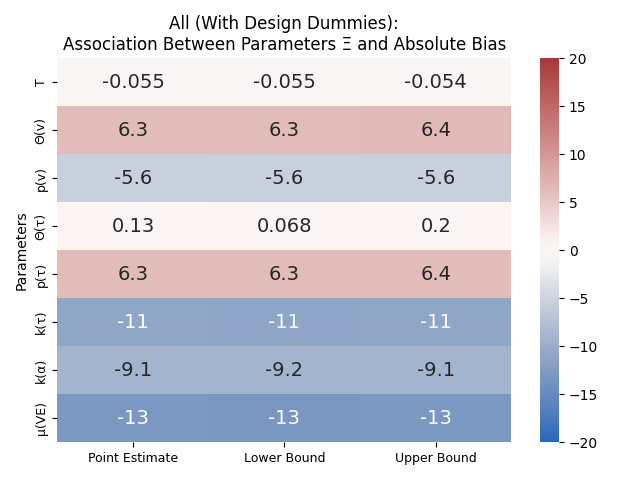
\includegraphics[scale=0.5]{VEMethod_Drivers1b_FEest_Li_Heatmap.png}
	\end{figure}
\end{frame}

\end{document}